\subsection{FPerf: An iProbe Application for Hardware Event Profiling}
\label{sec:imp:configure}


\begin{figure}[t]
    \begin{center}
      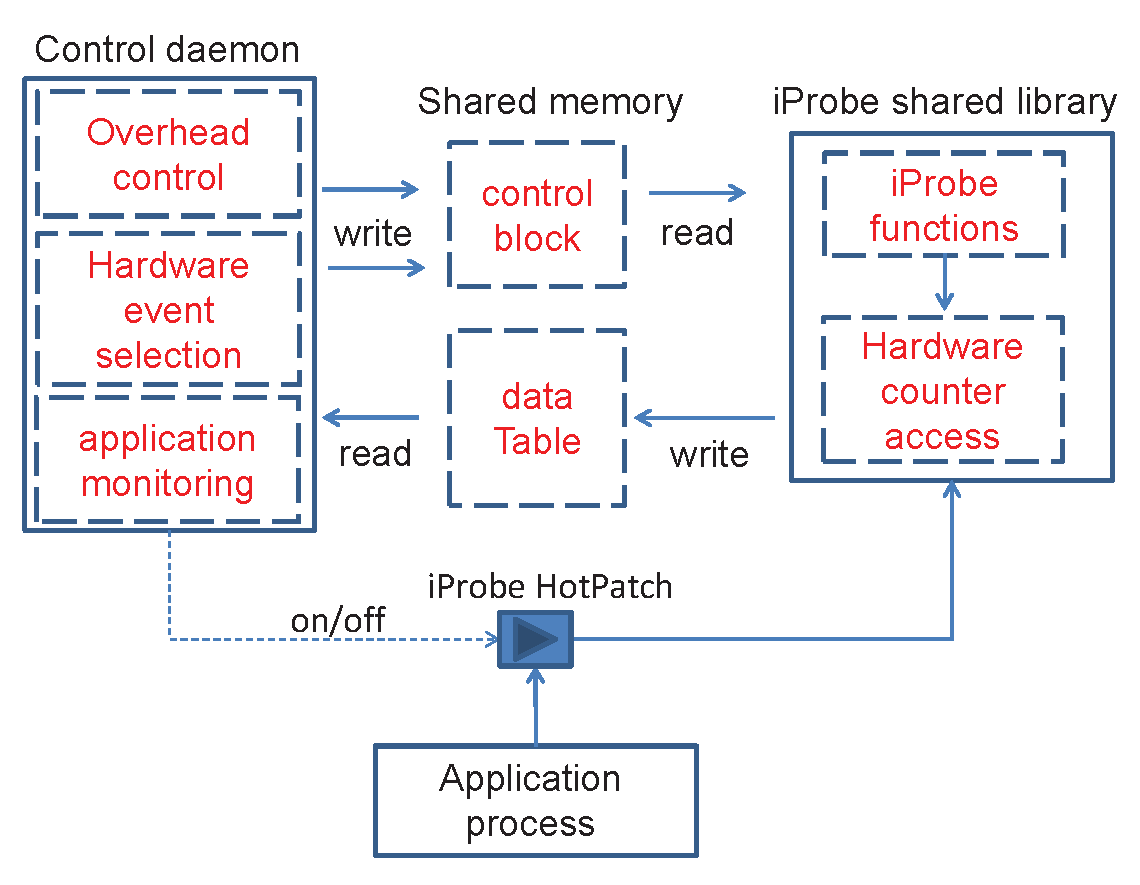
\includegraphics[width=0.8\textwidth]{iprobe/Images/sysdesign2.eps}
      \caption{Overview of \textit{FPerf}: Hardware Event Profiler based on iProbe.}
      \label{fig:implement}
    \end{center}
\end{figure}

%In this section we showcase iProbe's strength as a tool building infrastructure.  
We used iProbe to build \emph{FPerf}, an automatic function level hardware event profiler.  
FPerf uses iProbe to provide an automated way to gather hardware performance information at 
application function granularity.
%We used iProbe to build a hardware counter profiling tool called {\em FPerf}.

Hardware counters provide low-overhead access to a wealth of detailed performance information related to CPU's functional units, caches and main memory etc.
Using iProbe's all function profiling, we capture the hardware performance counters at the entry and exit of each function.
%\textit{FPerf} offers fine-grained hardware counter monitor profiling at application function level.
To control the perturbation on applications and the run-time system, \textit{FPerf} also implements a control mechanism to constraint the function profiling overhead within a budget configured by users.

Figure \ref{fig:implement} summarizes \textit{FPerf} implementation. 
It includes a control daemon and an iProbe shared library with customized instrumentation functions. 
The iProbe instrumentation functions access hardware performance counters (using PAPI\cite{papi} in the implementation) at the entry and exit of a selected target function to get the number of hardware events occurring during the function call. 
We define this process as taking one sample. 
Each selected function has a budget quota.
After taking one sample, the instrumentation functions decrease the quota for that application function by one. 
When its quota reaches zero, iProbe does not take sample anymore for that function.


The daemon process controls run-time iProbe profiling through shared memory communication.  
There are two shared data structures for this purpose: a shared control block where the daemon process passes to the iProbe instrumentation functions the profiling quota information, and a shared data table where the iProbe instrumentation functions record the hardware event information for individual function calls. 
When iProbe is enabled, i.e., the binary is HotPatched, daemon periodically collects execution data. 
We limit the total number of samples we want to collect in each time interval to restrict the overhead.  
This limitation is important because in software execution, the function call happens very frequently. 
For example, even with test data size input, the SPEC benchmarks generate 50MB-2GB trace files if we log the records for each function call. 
%Therefore, we initially assign a limitation for the total number of samples to limit the trace log size. 
%In the first 1s, when one function is called; we assign a minimum 1 sample quota for this function. 
%After that, we do not sample other calls to the function. But we keep counting the call number of the function. 
%After the initial 1s, the daemon process assigns the rest total sample quota for each selected application functions proportionally according to the previous call frequency of the functions. 
Functions that are frequently called will get more samples. 
Each selected function cannot take more samples than its assigned quota. 
The only exception happens when one function has never been called before; we assign a minimum one sample quota for each selection function. 
And we pick a function with quota that has not been used up, and decrease the quota of it by one. 
The above overhead control algorithm is a simplified Leaky Bucket algorithm~\cite{lba} originally for traffic shaping in networks. Other overhead control algorithms are also under consideration.

The control daemon also enables/disables the iProbe HotPatching based on user-defined application monitoring rules.
Essentially, this is an external control role on when and what to trace a target application with iProbe.
A full discussion of the hardware event selection scheme and monitoring rule design is beyond the scope of this paper. 
